\documentclass[tikz]{standalone}

\usetikzlibrary{angles}

\colorlet{FilledSurface}{blue!20}
\colorlet{FilledSurfaceGroupOne}{blue!20}
\colorlet{FilledSurfaceGroupTwo}{red!20}
\colorlet{FilledSurfaceGroupThree}{green!20}
\colorlet{FilledSurfaceGroupFour}{magenta!20}
\colorlet{FormulaBackground}{green!10}
\colorlet{FormulaFrame}{green}

\usetikzlibrary{calc}

\begin{document}
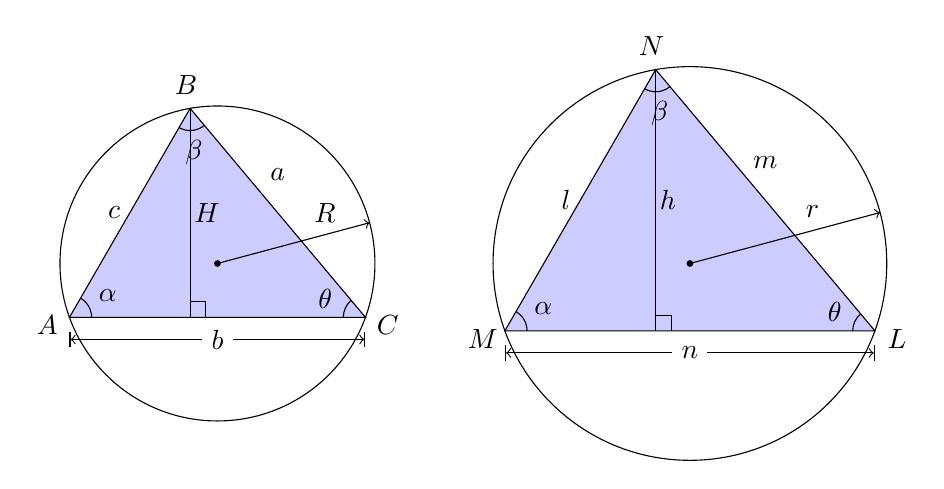
\begin{tikzpicture}

    \def\offset{0.3}
    % Angles used by both triangles
    \def\angleOne{200}
    \def\angleTwo{100}
    \def\angleThree{340}

    % ---------- Triángulo 1

    \def\tOneCircumradius{2}

    \coordinate (tOneCenter) at (0, 0);
    \draw (tOneCenter) circle (\tOneCircumradius);
    \coordinate (tOneA) at ($(tOneCenter) + (\angleOne:\tOneCircumradius)$);
    \coordinate (tOneB) at ($(tOneCenter) + (\angleTwo:\tOneCircumradius)$);
    \coordinate (tOneC) at ($(tOneCenter) + (\angleThree:\tOneCircumradius)$);
    \draw[fill=FilledSurfaceGroupOne]
    (tOneA) -- node [left] {$c$}
    (tOneB) --  node [above = 8pt] {$a$}
    (tOneC) -- cycle;
    \draw[color = black,|<->|] ($(tOneA)!8pt!-90:(tOneC)$) to node [fill=white] {$b$} ($(tOneC)!8pt!90:(tOneA)$);

    \node at ($(tOneCenter) + (\angleOne:\tOneCircumradius + \offset)$) {$A$};
    \node at ($(tOneCenter) + (\angleTwo:\tOneCircumradius + \offset)$) {$B$};
    \node at ($(tOneCenter) + (\angleThree:\tOneCircumradius + \offset)$) {$C$};

    % Show angles
    \path pic [draw, angle radius = 8pt, angle eccentricity = 2pt, pic text={$\alpha$}] {angle = tOneC--tOneA--tOneB};
    \path pic [draw, angle radius = 8pt, angle eccentricity = 2pt, pic text={$\theta$}] {angle = tOneB--tOneC--tOneA};
    \path pic [draw, angle radius = 8pt, angle eccentricity = 2pt, pic text={$\beta$}] {angle = tOneA--tOneB--tOneC};
    \coordinate (tOneBProj) at ($(tOneA)!(tOneB)!(tOneC)$);
    \draw (tOneB) -- node [right=-2pt] {$H$} (tOneBProj);
    \path pic [draw, angle radius=2mm] {right angle = tOneB--tOneBProj--tOneC};

    % Show center of circle
    \draw[fill=black] (tOneCenter) circle (1pt);

    % Show radius
    \def\angle{15}
    \draw[->] (tOneCenter) -- node [above right = 4pt] {$R$} ($(tOneCenter) + (\angle:\tOneCircumradius)$);

    % ---------- Triángulo 2

    \def\tTwoCircumradius{2.5}

    \coordinate (tTwoCenter) at (6, 0);
    \draw (tTwoCenter) circle (\tTwoCircumradius);
    \coordinate (tTwoM) at ($(tTwoCenter) + (\angleOne:\tTwoCircumradius)$);
    \coordinate (tTwoN) at ($(tTwoCenter) + (\angleTwo:\tTwoCircumradius)$);
    \coordinate (tTwoL) at ($(tTwoCenter) + (\angleThree:\tTwoCircumradius)$);
    \draw[fill=FilledSurfaceGroupOne]
    (tTwoM) -- node [left] {$l$}
    (tTwoN) --  node [above = 8pt] {$m$}
    (tTwoL) -- cycle;
    \draw[color = black,|<->|] ($(tTwoM)!8pt!-90:(tTwoL)$) to node [fill=white] {$n$} ($(tTwoL)!8pt!90:(tTwoM)$);

    \node at ($(tTwoCenter) + (\angleOne:\tTwoCircumradius + \offset)$) {$M$};
    \node at ($(tTwoCenter) + (\angleTwo:\tTwoCircumradius + \offset)$) {$N$};
    \node at ($(tTwoCenter) + (\angleThree:\tTwoCircumradius + \offset)$) {$L$};

    % Show angles
    \path pic [draw, angle radius = 8pt, angle eccentricity = 2pt, pic text={$\alpha$}] {angle = tTwoL--tTwoM--tTwoN};
    \path pic [draw, angle radius = 8pt, angle eccentricity = 2pt, pic text={$\theta$}] {angle = tTwoN--tTwoL--tTwoM};
    \path pic [draw, angle radius = 8pt, angle eccentricity = 2pt, pic text={$\beta$}] {angle = tTwoM--tTwoN--tTwoL};
    \coordinate (tTwoNProj) at ($(tTwoM)!(tTwoN)!(tTwoL)$);
    \draw (tTwoN) -- node [right=-2pt] {$h$} (tTwoNProj);
    \path pic [draw, angle radius=2mm] {right angle = tTwoN--tTwoNProj--tTwoL};

    % Show center of circle
    \draw[fill=black] (tTwoCenter) circle (1pt);

    % Show radius
    \def\angle{15}
    \draw[->] (tTwoCenter) -- node [above right=4pt] {$r$} ($(tTwoCenter) + (\angle:\tTwoCircumradius)$);

\end{tikzpicture}
\end{document}


